\clearpage

\appendix

\section{Appendix A: Data Pipelines}
\label{sec:appendix-a-data-pipelines}

\textbf{NOTE the content of this table and illustration are outdated}

In table \ref{tab:data-pipelines} all the data pipelines are listed with a description of their operation. In figure \ref{fig:data-pipelines} the pipelines are visualized (TODO: outdated). Many data pipelines are relatively straightforward and don't need further explanation than listed in the table.

% Please add the following required packages to your document preamble:
% \usepackage{booktabs}
% \usepackage{graphicx}
\begin{table}[h!]
\resizebox{\textwidth}{!}{%
\begin{tabular}{@{}p{0.25\linewidth}llp{0.6\linewidth}@{}}
\toprule
Name &
  Source &
  Destination &
  Description \\ \midrule \midrule
Ingest Accelerometer &
  \begin{tabular}[c]{@{}l@{}}Landing\\ Cloud Storage (jsonlines)\end{tabular} &
  \begin{tabular}[c]{@{}l@{}}Landing\\ BigQuery\\ \textit{raw\_accelerometer}\end{tabular} &
  Loads raw records from Cloud Storage into BigQuery table. \\ \midrule
Ingest GPS &
  \begin{tabular}[c]{@{}l@{}}Landing\\ Cloud Storage (jsonlines)\end{tabular} &
  \begin{tabular}[c]{@{}l@{}}Landing\\ BigQuery\\ \textit{raw\_gps}\end{tabular} &
  Loads raw records from Cloud Storage into BigQuery table. \\ \midrule
Ingest Wegdeel &
  \begin{tabular}[c]{@{}l@{}}External\\ Postgis\end{tabular} &
  \begin{tabular}[c]{@{}l@{}}Landing\\ BigQuery\\ \textit{raw\_wegdeel}\end{tabular} &
  Loads road sections (wegdeel) from Postgis database into BigQuery table. \\ \midrule
Ingest Frames Labels &
  \begin{tabular}[c]{@{}l@{}}Landing\\ Cloud Storage (txt)\end{tabular} &
  \begin{tabular}[c]{@{}l@{}}Landing\\ BigQuery\\ \textit{raw\_frames\_labels}\end{tabular} &
  Loads manually label annotations into BigQuery table. \\ \midrule
Ingest Label Lookup &
  \begin{tabular}[c]{@{}l@{}}Landing\\ Cloud Storage (txt)\end{tabular} &
  \begin{tabular}[c]{@{}l@{}}Landing\\ BigQuery\\ \textit{raw\_label\_lookup}\end{tabular} &
  Loads manually label definitions into BigQuery table. \\ \midrule \midrule
Determine Trips &
  \begin{tabular}[c]{@{}l@{}}Landing\\ BigQuery\\ \textit{raw\_gps}\end{tabular} &
  \begin{tabular}[c]{@{}l@{}}Staging\\ BigQuery\\ \textit{stg\_gps}, \textit{stg\_trips}\end{tabular} &
  Parses from GPS records distinct trips the car has travelled (further described below). \\ \midrule
Snap Trips to Roads &
  \begin{tabular}[c]{@{}l@{}}Staging\\ BigQuery\\ \textit{stg\_trips}\\ \\ External\\ Bing\end{tabular} &
  \begin{tabular}[c]{@{}l@{}}Staging\\ BigQuery\\ \textit{stg\_trips\_snapped}\end{tabular} &
  Snap the preprocessed GPS records to actual roads (further described below). \\ \midrule
Filter Road Sections &
  \begin{tabular}[c]{@{}l@{}}Landing\\ BigQuery\\ \textit{raw\_wegdeel}\end{tabular} &
  \begin{tabular}[c]{@{}l@{}}Staging\\ BigQuery\\ \textit{stg\_road\_section}\end{tabular} &
  Filter the road sections that are actually in use. \\ \midrule
Create Label Lookup &
  \begin{tabular}[c]{@{}l@{}}Landing\\ BigQuery\\ \textit{raw\_label\_lookup}\end{tabular} &
  \begin{tabular}[c]{@{}l@{}}Staging\\ BigQuery\\ \textit{stg\_label\_lookup}\end{tabular} &
  Converts ingested definitions to lookup table in order to join with annotated frames.\\ \midrule
Video to Frames &
  \begin{tabular}[c]{@{}l@{}}Landing\\ Cloud Storage (mov)\end{tabular} &
  \begin{tabular}[c]{@{}l@{}}Staging\\ Cloud Storage (jpg)\end{tabular} &
  Extracts separate frames from the recorded video (1 frame per second).\\ \midrule
Video to Frames Bootstrap &
  &
  &
  Spawns off separate jobs to process all video files in parallel.\\ \midrule \midrule
Link Trip Coordinates with Road Sections &
  \begin{tabular}[c]{@{}l@{}}Staging\\ BigQuery\\ \textit{stg\_trips\_snapped}\\ \\ Staging\\ BigQuery\\ \textit{stg\_road\_section}\end{tabular} &
  \begin{tabular}[c]{@{}l@{}}Production\\ BigQuery\\ \textit{mrt\_trips}\end{tabular} &
  Joins the snapped trips with the cleaned road sections from the BGT. \\ \midrule
Calculate Road Section Windows &
  \begin{tabular}[c]{@{}l@{}}Production\\ BigQuery\\ \textit{mrt\_trips}\end{tabular} &
  \begin{tabular}[c]{@{}l@{}}Production\\ BigQuery\\ \textit{mrt\_road\_section\_windows}\end{tabular} &
  Calculates timestamps (windows) when each road section was entered/exited per trip. \\ \midrule
Load Frames Labels &
  \begin{tabular}[c]{@{}l@{}}Landing\\ BigQuery\\ \textit{raw\_frames\_labels}\\ \\ Staging\\ BigQuery\\ \textit{stg\_label\_lookup}\end{tabular} &
  \begin{tabular}[c]{@{}l@{}}Production\\ BigQuery\\ \textit{mrt\_frames\_labels}\end{tabular} &
  Joins annotated frames with lookup table. \\ \midrule 
Load Frames Metadata &
  \begin{tabular}[c]{@{}l@{}}Production\\ Storage\end{tabular} &
  \begin{tabular}[c]{@{}l@{}}Production\\ BigQuery\\ \textit{mrt\_frames\_metadata}\end{tabular} &
  Creates a metadata table on the extracted frames (e.g. source video, timestamp and size). \\ \midrule 
Ingest Experiment Labels &
  \begin{tabular}[c]{@{}l@{}}External\end{tabular} &
  \begin{tabular}[c]{@{}l@{}}Production\\ BigQuery\\ \textit{mrt\_experiment\_labels}\end{tabular} &
  Ingests separate labels annotated by experiment runs into BigQuery. \\ \midrule 
Anonymize &
  \begin{tabular}[c]{@{}l@{}}Staging\\ Cloud Storage (jpg)\end{tabular} &
  \begin{tabular}[c]{@{}l@{}}Production\\ Cloud Storage (jpg)\end{tabular} &
  Automatically detect PII data and blur the detected objects.\\ \midrule
Anonymize Bootstrap &
  &
  &
  Spawns off separate jobs to process all source files in parallel.\\ \bottomrule
\end{tabular}%
}
\caption{Overview of all the different data pipelines.}
\label{tab:data-pipelines}
\end{table}

\begin{figure}[h!]
\begin{center}
\makebox[\textwidth][c]{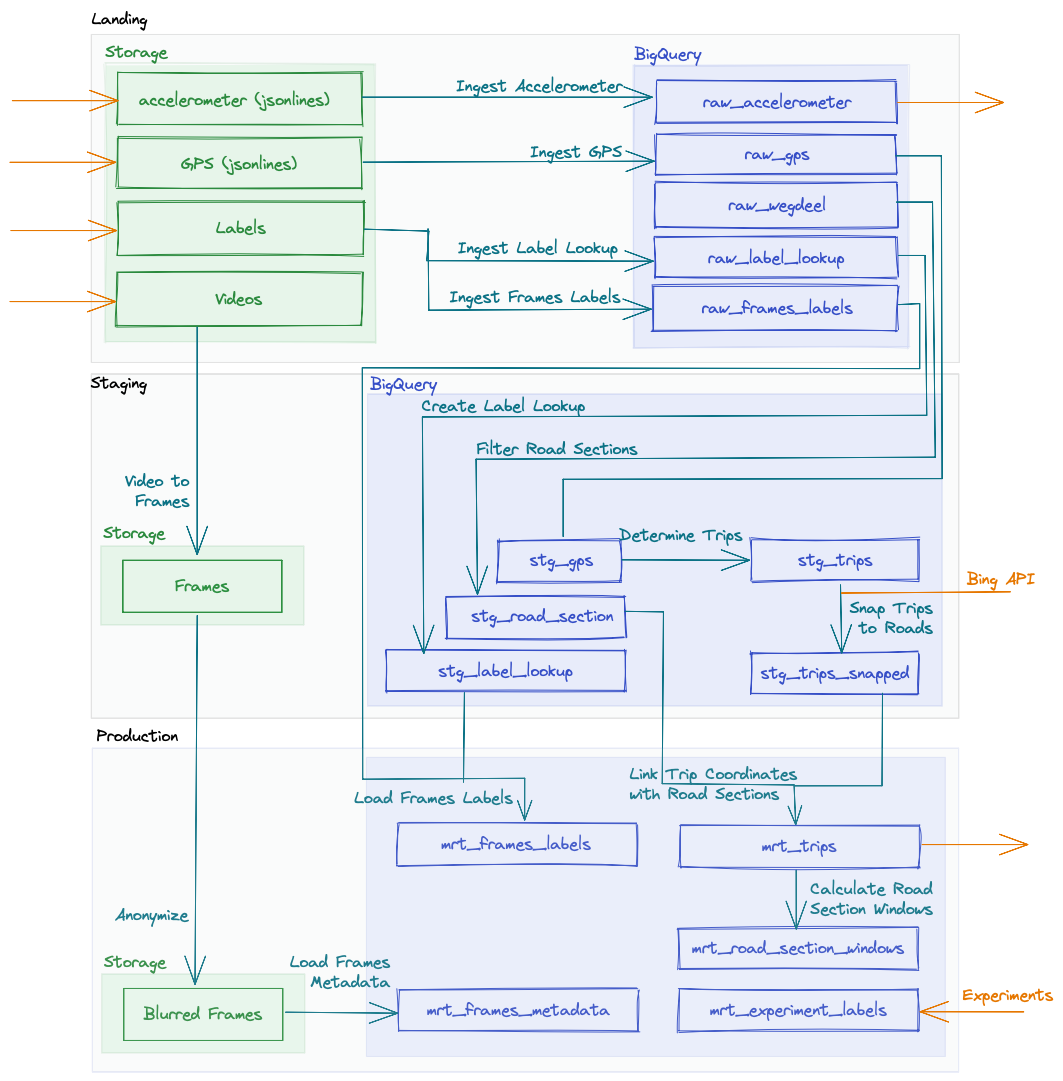
\includegraphics[width=1.2\textwidth,keepaspectratio]{images/4_data/data-pipelines.png}}
\end{center}
\caption{Visual overview of the various Data Pipelines.}
\label{fig:data-pipelines}
\end{figure}
